\chapter{Charged Lepton Flavor Violation}
\textit{This chapter offers a concise overview of the fundamental theoretical and experimental components essential to understand the objectives of the Mu2e experiment at Fermilab and the work conducted for this Thesis. The introduction to the Standard Model and certain extensions serves to justify the investigation of Charged Lepton Flavor Violation (CLFV), since it would be a clear signal of new physics beyond the current theories. Fundamental bibliography for this chapter can be found in Ref. \cite{Bernstein_2013} and \cite{clfv_signorelli}.}
\section{Theoretical Introduction}
\subsection{The Standard Model}
The Standard Model provides an excellent description of elementary particles and their interactions. It describes three out of four the fundamental forces known to this day: electromagnetism interaction, weak interaction and strong interaction. This theory is based on the gauge symmetry group $U(1)_Y \times SU(2)_L \times SU(3)_C$. The first two terms describe the electroweak interaction, $Y$ indicates the hypercharge and $L$ refers to the fact that this acts only on the left handed components of the fields. The last term describes the strong interaction and $C$ indicates the color charge.
The Standard Model contains 25 elementary fields, shown in Fig. \ref{fig:sm}.

\begin{figure}[!h]
\centering
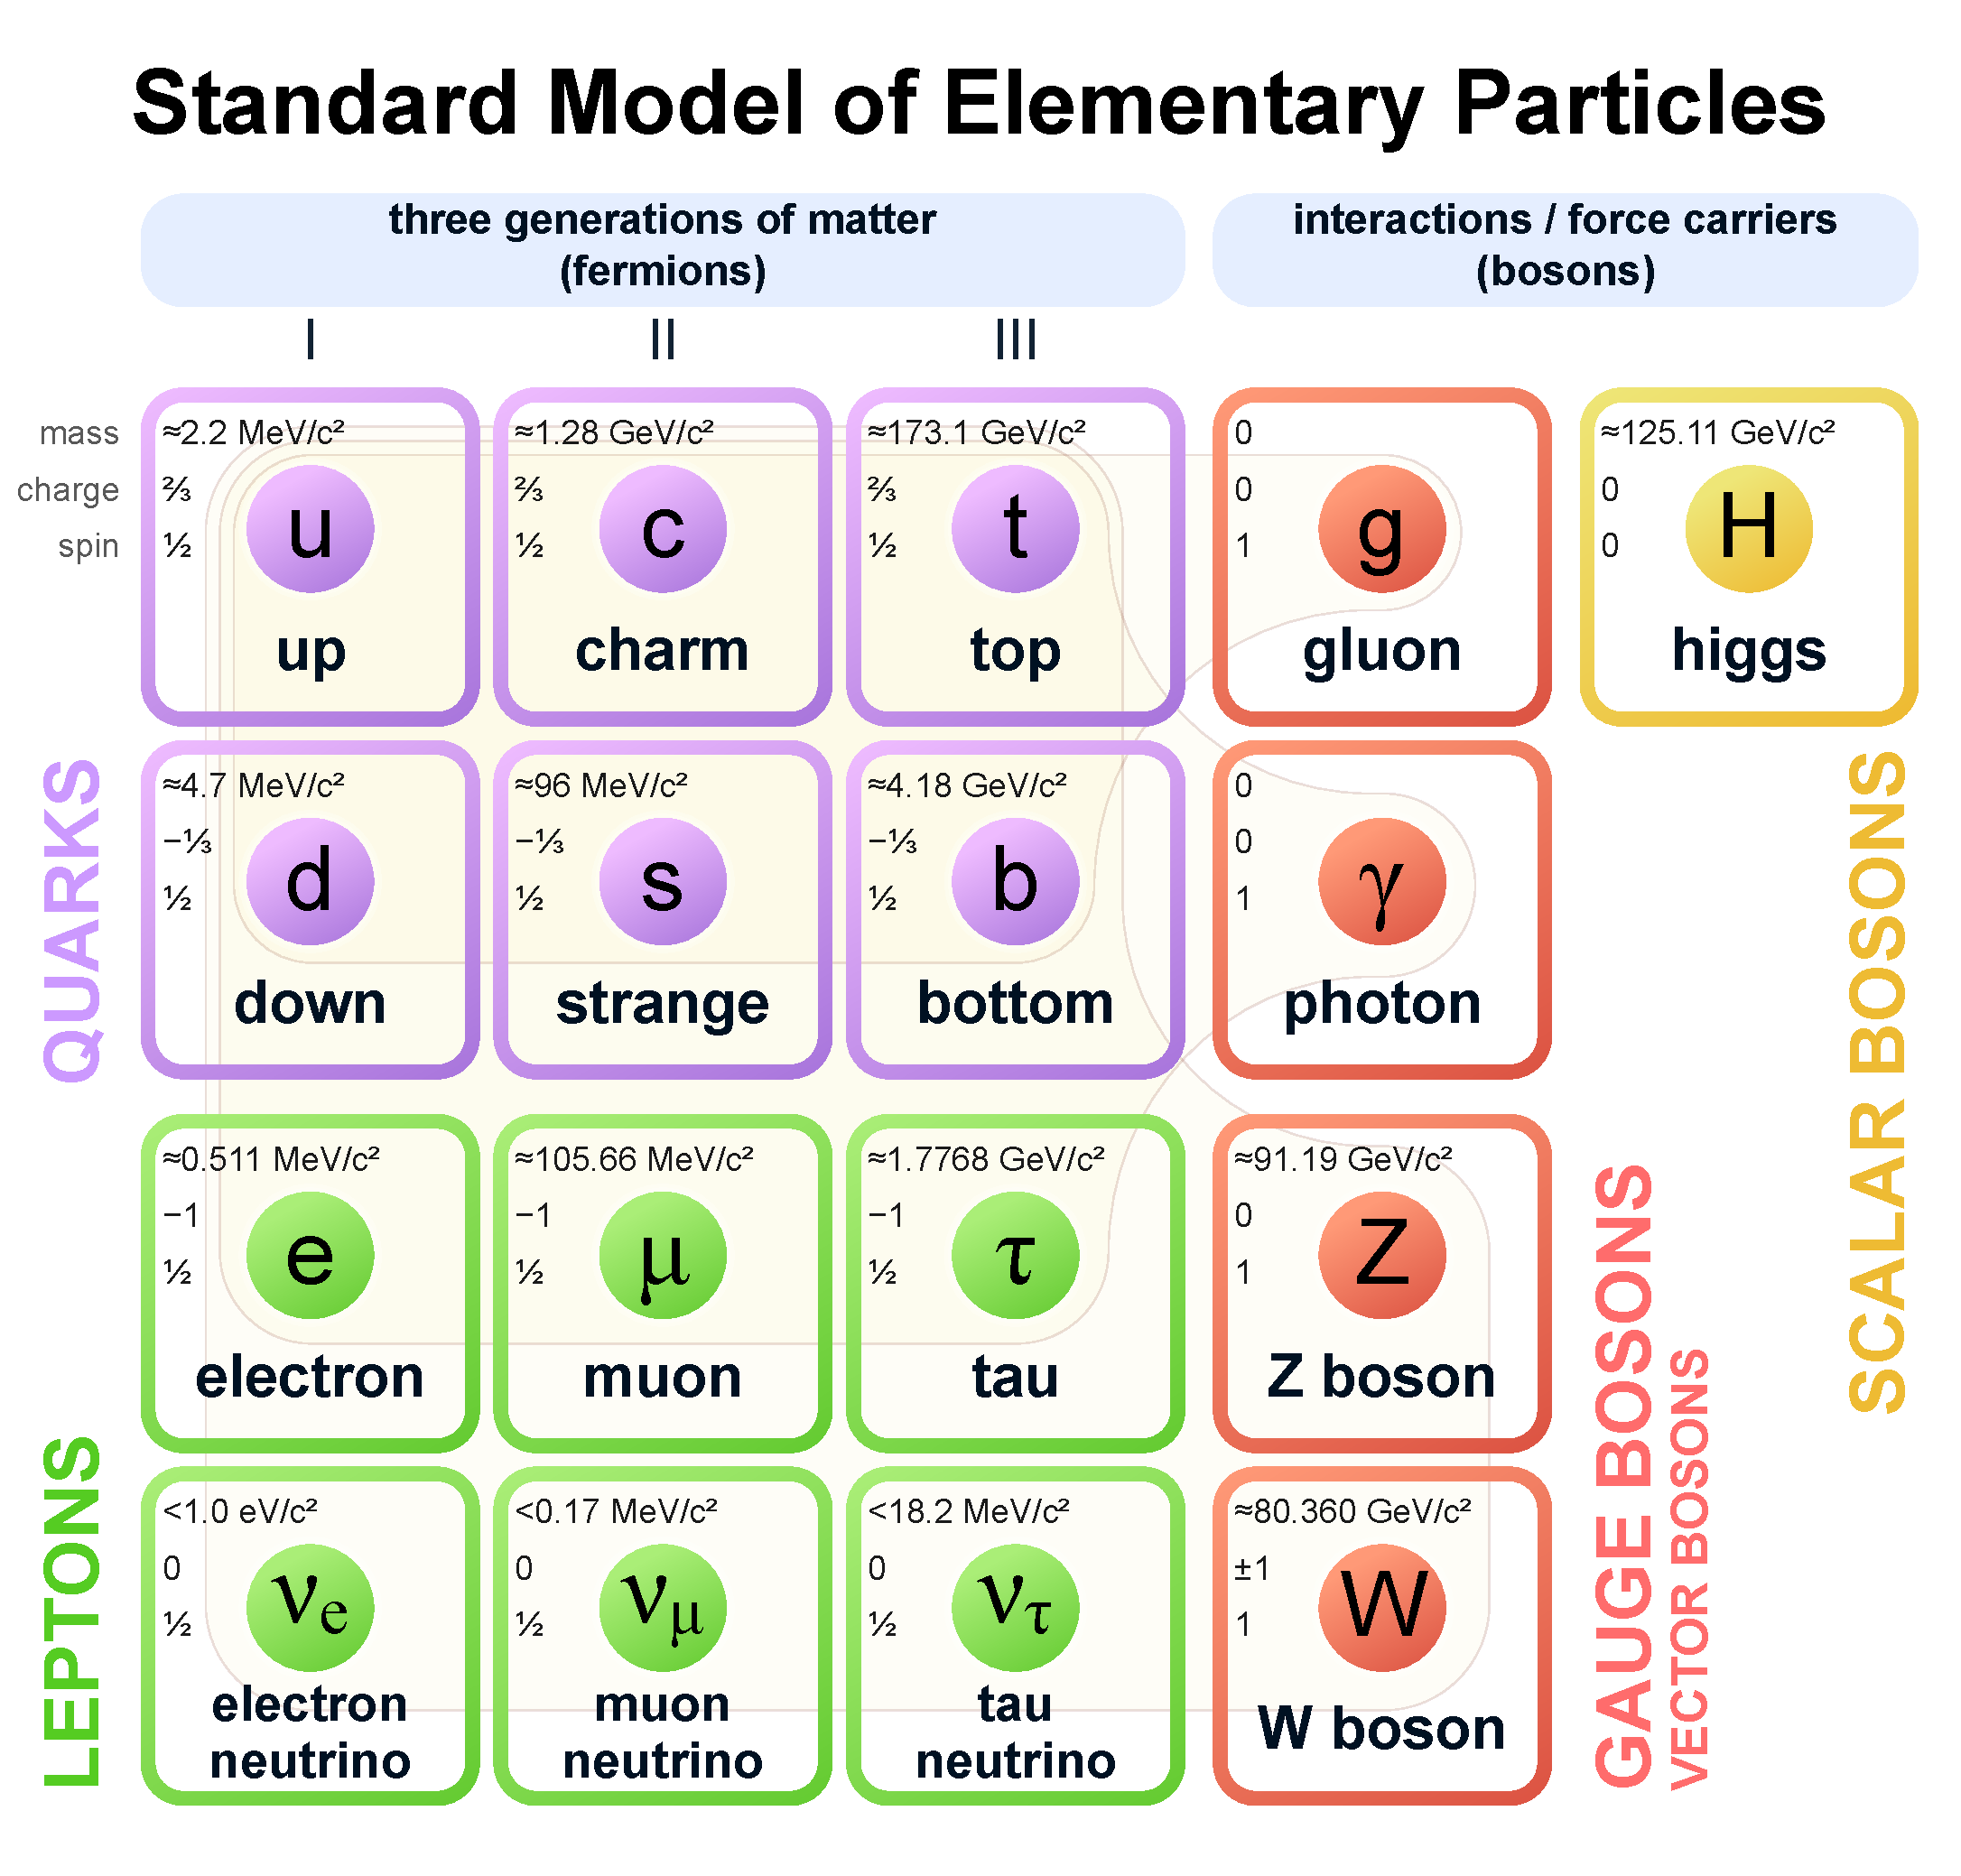
\includegraphics[width =0.8\textwidth]{figures/pdf/Standard_Model_of_Elementary_Particles.pdf}
\caption{Elementary particles of the Standard Model.}
\label{fig:sm}
\end{figure}


\subsubsection{Bosons}\label{bosons}
A boson is a particle with zero or integer spin, which follows Bose-Einstein statistics.
There are twelve fundamental bosons, that are the mediators of interactions as the $\gamma$, $Z$, $W^{\pm}$ for the electroweak interaction and as the eight gluons for the strong interaction.
The Higgs is a complex scalar weak isospin doublet that is responsible for the mechanism through which fermions and
bosons acquire mass and also explains the origin of $U (1)_{EM}$ through the spontaneous
symmetry breaking of the $SU (2)_L \times SU (1)_Y$ in the electroweak sector. Also mesons, that are composed of a quark and antiquark pair, are bosons. Bosons can be either massive, as $Z$, Higgs and $W^{\pm}$, or massless, as the photon and gluons.

\subsubsection{Fermions}
A fermion is a particle characterized by a non-integer spin, i.e. $1/2$, $3/2$ and follows the Fermi-Dirac statistics. The Pauli exclusion principle must be respected. Fermions are divided in two categories, leptons and quarks, depending on the forces through which they interact.  The arrangement of fermions into three generations is dictated by various properties, including mass among other properties, with more massive particles assigned to higher generations, as depicted in Fig.\ref{fig:sm}. Particles of the second and third generations exhibit instability and decay into first-generation particles. Leptons do not interact through strong interaction because they are not color charged, so they interact only via weak and electromagnetic interaction. They are categorized into two groups based on the electric charge: $e$, $\mu$, $\tau$ are the charged leptons and $\nu_e$, $\nu_{\mu}$, $\nu_{\tau}$ are the neutral ones. These particles form doublets of flavour. Neutrinos, due to their neutral nature, interact only weakly so their detection is extremely challenging. The six quarks participate in all known interactions. The known quarks are, in ascending order of mass and generation: up ($u$) and down ($d$), strange ($s$) and charm ($c$), bottom ($b$) and top ($t$) and their antiparticles. They primarily interact with each other through the strong force by gluons exchange. Free quarks have never been observed due to confinement, since they carry color charge. Confinement of quarks is a fundamental aspect of the theory of quantum chromodynamics (QCD) which describes the strong nuclear force. Quarks combine to form color-neutral particles known as hadrons, classified into baryons and mesons. Baryons consist of an odd number of quarks, while mesons, as mentioned in Subsection \ref{bosons}, are composed of a quark and an antiquark. Since quarks have weak electric charge and isospin, they can interact with each other and other fermions through weak and electromagnetic interactions.

\subsection{History of flavor}
The concept of flavor, namely the presence of three duplicates for every family of elementary fermions, is a fundamental aspect in particle physics. This principle is implemented within the Standard Model by introducing three copies of the gauge representations of fermion fields. This view began to take shape in the late 1940s. The origin can be traced back to the experiment conducted by Conversi, Pancini and Piccioni in 1947. These experiment revealed that negative muons, called at that time $mesotrons$, did not undergo nuclear capture as expected. They decayed in electrons, similarly to positive muons, therefore they could not be Yukawa particles. In the same year, Powell and his group identified a two-step decay process ($\pi \rightarrow \mu \rightarrow e$), distinguishing the pion from the muon. Bruno Pontecorvo suggested that the muon could be a sort of $isomer$ of the electron, leading to the idea of a second generation of elementary fermions. Rochester and Butler discovered unusual events in cosmic rays pictures, later identified as $V-particles$ (later discovered that they originated from neutral kaons). This was the first hint of the existence of a second generation of quarks. In 1950 the search for decay $\mu \rightarrow e \gamma$ began. This decay was not found, leading to the principle of conservation of leptons. On the hadron side, the second generation of quarks was established in the mid-70s, involving the GIM mechanism and the discovery of the charm quark. Meanwhile, on the leptonic side, the upper limit on the branching ratio of $\mu^+ \rightarrow  e^+ \gamma$ was set in 1955. The discovery of parity violation in the late 1950s suggested the weak interaction is mediated by bosons. \textit{Feinberg started thinking that $\mu^+ \rightarrow  e^+ \gamma$ could occur at a level of $10^{-4}$ if the bosons existed, through a loop with neutrino and a boson}. This lead to the two-neutrino hypothesis, suggesting that the neutrino coupled to the muon differs from that coupled to the electron, thereby prohibiting $\mu^+ \rightarrow  e^+ \gamma$. The existence of two neutrinos was verified at Brookhaven National Laboratory, with the scattering of two neutrinos coming from $\pi$, that produced only muons. After the observation of CP violation in neutral kaon decay, a third generation of quarks was hypothesized. After the discoveries of the $\tau$ (1976), the $b$ quark (1977), $t$ quark (1995) and $\nu_{\tau}$ (2000), a complete picture was achieved and the concept of flavor was consolidated in the Standard Model.


\subsection{Overview of CLFV}
There are three different lepton flavors: the electron-lepton number $L_e$, the muon-lepton number $L_{\mu}$ and the tau-lepton number $L_{\tau}$. In Table \ref{tab:leptons}, the quantum numbers assigned to each lepton are displayed.
 \begin{center}  
\begin{table}[!h]
\centering
\renewcommand{\arraystretch}{1.5}
\begin{tabular}{c c c c}
\hline
Lepton & $L_e$ & $L_{\mu}$ & $L_{\tau}$\\
\hline
$e^-/e^+$ & $+1 \ /-1$ & 0 & 0 \\
$\nu_{e}/\bar{\nu}_{e}$ & $+1 \ /-1$ & 0 & 0 \\
$\mu^-/\mu^+$ & 0 & $+1 \ /-1$ & 0 \\
$\nu_{\mu}/\bar{\nu}_{\mu}$ & 0 & $+1 \ /-1$ & 0 \\
$\tau^-/\tau^+$ & 0 & 0 & $+1 \ /-1$\\
$\nu_{\tau}/\bar{\nu}_{\tau}$ & 0 & 0 & $+1 \ /-1$ \\
\hline
\end{tabular}
\caption{Lepton numbers assigned to neutrinos and charged leptons.}
\end{table}\label{tab:leptons}
\end{center}
In the Standard Model (SM) defined with massless left-handed neutrinos, Lepton Flavor (LF) is a conserved quantity, Ref. \cite{universe8060299}. Experimental observations have demonstrated that, as they travel, neutrinos exhibit flavor oscillations, which implies that they must have non-zero masses and mixing angles. This phenomenon represents also a violation of the conservation of the lepton flavor. The Standard Model, while successful in many aspects, fails to explain phenomena like neutrino masses and the consequent flavor oscillations. Since neutrinos get their masses through renormalizable Yukawa interactions
with the Higgs, the predicted CLFV transitions are suppressed by sums over $(\Delta m^2_{i j}/M^2 _W)^2$, as calculated in Ref. \cite{MARCIANO1977303} and as shown in Section \ref{massiveneutrinos}, where $\Delta m^2_{ij}$ is mass-squared difference between the neutrino mass eigenstates $i$, $j$ and $M_W$ is the $W$ boson mass. The neutrino mass difference is very small ($\Delta m^2 _{i j} \leq 10^{-3}$ eV$^2$) with respect to the $W$ boson mass so the expected branching ratios reach unmeasurable values, below $10^{-50}$. Experimental studies of the lepton flavor violating process could open a window to new physics. Moreover, lepton flavor constitutes an accidental symmetry within the SM, not related to the gauge structure of the theory but coming
from its particle content, especially from the absence of RH neutrinos. Minor deviations from the Standard Model can easily give rise to extra occurrences of lepton flavor violation, leading to notable rates of CLFV.
There are various extensions of the Standard Model that could potentially be examined in the upcoming experimental searches for CLFV.
In Section \ref{leptonsector}, I will talk about lepton sector and how the lepton numbers are conserved. In Section \ref{massiveneutrinos}, a brief introduction of CLFV with massive neutrinos will be given.
In Section \ref{2higgs} and in Section \ref{susy}, I present a short discussion on Two Higgs Doublet Model and the CLFV in Super-symmetry respectively.
\subsection{Lepton sector in Standard Model}\label{leptonsector}
In the SM, only one Higgs field $\Phi$ exists. The fermions masses and the mixing term arise from the couplings of fermions with Higgs field. In the following, I will call the left-handed $i$-th quarks doublets and leptons doublets as $Q_{L,i}=(u_{L,i} \ d_{L,i})^T$ and $L_{L,i}=(\nu_{L,i} \ e_{L,i})^T$: $u_i$ will be the up-type quark, $d_i$ the down-type quark, $\nu_i$ the neutrino and $e_i$ the charged lepton. These are $SU(2)$ doublets, while $u_{R,j}$, $d_{R,j}$ and $e_{R,j}$ will be the right-handed up-type, down-type quarks and the right charged lepton of the $j$-generation respectively. There is no right-handed neutrino. The Yukawa coupling of fermions with the Higgs field $\mathscr{L}_Y$ is the sum of two terms: $\mathscr{L}_e$ that describes the leptonic component (Eq.\ref{leptoniccomponent}) and $\mathscr{L}_q$ that describes the quark one (Eq.\ref{quarkcomponent}).
\begin{equation}\label{leptoniccomponent}
    -\mathscr{L}_e=\left(Y_e\right)_{i j} \bar{L}_{L i} e_{R j} \Phi+ \text{ h.c. }
\end{equation}
\begin{equation}\label{quarkcomponent}
        -\mathscr{L}_q=\left(Y_u\right)_{i j} \bar{Q}_{L i} u_{R j} \widetilde{\Phi}+\left(Y_d\right)_{i j} \bar{Q}_{L i} d_{R j} \Phi+\text { h.c. }
\end{equation}

where the term $Y_f \ (f  =  u,d,e)$ describe the 3$\times$3 Yukawa complex matrices. $\widetilde{\Phi} \equiv i \tau_2 \Phi^*$ is the conjugate Higgs field. The mass terms of fermions, characterized by the $m_f \bar{f}_L f_R$ form, originate from the breaking of the $SU(2)_L \times U(1)$ symmetry caused by the vacuum expectation value of the Higgs field, as in Eq.\ref{higgs}.
\begin{equation}\label{higgs}
\langle\Phi\rangle=\frac{1}{\sqrt{2}}\left(\begin{array}{l}
0 \\
v
\end{array}\right) \qquad v \simeq 246 \mathrm{GeV}
\end{equation}
The fermion mass is given by:
\begin{equation}
\left(m_f\right)_{i j}=\frac{v}{\sqrt{2}}\left(Y_f\right)_{i j} \qquad f=u, d, e
\end{equation}
Since a right-handed neutrino does not appear in the Lagrangian, neutrinos have no mass, as it is formulated in the SM. The Yukawa matrices can be diagonalized through unitary rotations of the fields, as it follows:
\begin{equation}
Y_f=V_f \hat{Y}_f U_f^{\dagger} \qquad f=u, d, e
\end{equation}
where $ \hat{Y}_f $ is the diagonal Yukawa matrix. It is possible to label fermions in the rotated basis as $f^{\prime}$, so $f_L=V_f f^{\prime}_L$ and $f_R=V_f f^{\prime}_R $. Since $V_f$ and $U_f$ are unitary, the rotation will not affect the neutral interactions term and the kinetic terms, as we can see in $\bar{f}_L \gamma^\mu f_L=\bar{f}_L \gamma^\mu\left(V_f^{\dagger} V_f\right) f_L=\bar{f}_L^{\prime} \gamma^\mu f_L^{\prime}$. The coupling between fermion and Higgs boson will be:
\begin{equation}
-\mathscr{L}_{h \bar{f} f}=\frac{(\hat{m}_f)_{i j}}{v} \bar{f}_{L i}^{\prime}f^{\prime}_{R j} h+\text{h.c.} \qquad f=u, d, e
\end{equation}
where $\hat{m}_f$ denotes the diagonalized mass matrix: it is clear that there are no flavor-violating terms.
In quark sector flavor-violation arises from the rotations in Eq.\ref{quarkviolation} in the charged-current interactions with the $W$ bosons:
\begin{equation}\label{quarkviolation}
\begin{array}{c}
      { \displaystyle 
\mathscr{L}_{C C}  =\frac{g}{\sqrt{2}}\left(\bar{u}_L \gamma^\mu d_L+\bar{\nu}_L \gamma^\mu e_L\right) W_\mu^{+}+\text {h.c.} }\\
 {\displaystyle=\frac{g}{\sqrt{2}}\left(\bar{u}^{\prime}_L \gamma^\mu\left(V_u^{\dagger} V_d\right) d_L^{\prime}+\bar{\nu}^{\prime}_L \gamma^\mu\left(V_\nu^{\dagger} V_e\right) e_L^{\prime}\right) W_\mu^{+}+\text {h.c.}}
\end{array}
\end{equation}

The violation comes from the fact that $V_u \neq V_d$. The mixing is controlled by the Cabibbo-Kobayashi-Maskawa matrix $V_{CKM}\equiv V^{\dagger}_u V_d $, Ref. \cite{PhysRevLett.10.531}. Meanwhile, as the lepton sector contains massless neutrinos, $V_{\nu}$ can be arbitrarily chosen as $V_{\nu}=V_e$. From the preceding discussions, it becomes evident that in the SM with massless neutrinos, there is no occurrence of LFV in any form. The Lagrangian $\mathscr{L}_Y$ is invariant under three indipendent global $U(1)$ rotations, resulting in the conservation of three lepton family numbers: $L_e$, $L_\mu$ and $L_\tau$. Furthermore, if the Yukawa coupling Lagrangian includes supplementary terms involving the lepton fields, flavor violation can occur in the lepton sector. Examples of such additions could be a neutrino mass term or a second Higgs doublet.

\subsection{CLFV in the Standard Model with massive neutrinos}\label{massiveneutrinos}
The first evidence against the hypotesis of massless neutrinos emerged with the solar neutrino problem. In the 1960s, the solar neutrino detection experiment at Homestake revealed that the observed number of solar neutrinos, generated by fusion in the Sun, was significantly lower than the anticipated value based on the standard solar model, given that the detector was only sensitive to $\nu_e$, Ref. \cite{PhysRevLett.20.1205}. Consistent results were replicated in subsequent experiments employing radiochemical and Cherenkov detectors, discovering neutrino oscillations. These oscillation firmly established non-zero neutrino masses. The lepton flavor-violating neutrino oscillations showed that the global $U(1)$ symmetries associated with the lepton family numbers are not fundamental symmetries. A correction to standard model is needed to include neutrino mass terms. This is possible adding a right-handed neutrino singlet $\nu_R$ or some non-renormalizable operators.
\\
In the first case, an additional term $\Delta \mathscr{L}_D$ to the Yukawa coupling should be introduced:
\begin{equation}
-\Delta \mathscr{L}_D=\left(Y_\nu\right)_{i j} \bar{L}_{L i} \nu_{Rj} \widetilde{\Phi}+\text { h.c. }
\end{equation}
Similarly to other fermions, a Dirac mass term $m_{\nu} \bar{\nu}_L \nu_R$ is generated through simmetry breaking:
\begin{equation}
\left(m_\nu^D\right)_{i j}=\frac{v}{\sqrt{2}}\left(Y_\nu\right)_{i j}
\end{equation}
In this case, the small neutrino masses can be explained only if a very small term $Y_\nu$ is considered ($\leq 10^{-12}$), Ref. \cite{clfv_signorelli}. This brings us considering the second hypotesis: adding non-renormalizable operators can introduce Majorana masses for left-handed neutrinos alone. The corresponding $\Delta \mathscr{L}_M$ can be written as:
\begin{equation}
-\Delta \mathscr{L}_M=\frac{1}{2}\left(m_\nu^M\right)_{i j} \overline{\nu_{L i}^C} \nu_{L j}+\text{ h.c.}
\end{equation}
where $\overline{\nu_{L }^C} $ is the charge-conjugated fields. This term violates lepton number and requires an operator of dimension 5, Ref. \cite{wein}, to be consistent with SM symmetries. A minimal Lagrangian is given by:
\begin{equation}
-\Delta \mathscr{L}_{M \text { eff}}=\frac{\mathcal{C}_{i j}}{\Lambda}\left(\overline{L_{L i}^C} \tau_2 \Phi\right)\left(\Phi^T \tau_2 L_{L j}\right)+\text { h.c.}
\end{equation}
where the $\Lambda$ term represents a mass scale characteristic of extra degrees of freedom and the $C_{ij}$ is an antisymmetric charge conjugation matrix. The corresponding Majorana mass term is:
\begin{equation}
\left(m_\nu^M\right)_{i j}=\frac{\mathcal{C}_{i j} v^2}{\Lambda}
\end{equation}
In this case, the small neutrino masses can be explained only if $\Lambda > > v$: this seems to appear more natural than the previous case. No matter how the extra neutrino mass factor is expressed precisely, a physical basis diagonalizing the mass matrix is determined, resulting in $V_{\nu} \neq V_e$ in Equation \ref{quarkviolation}. Lepton mixing is described by $U_{PMNS} \equiv V_{\nu}^{\dagger} V_e$, which is similar to the CKM matrix. The Pontecorvo-Maki-Nakagawa-Sakata (PMNS) matrix is the term that is typically used to refer to it. As it is in the basis diagonalizing charged lepton masses and it diagonalizes the neutrino mass matrix, $U_{PMNS}$ also explains the mixing between neutrino flavor eigenstates $\nu_{\alpha}$ and mass eigenstates $\nu_i$:
\begin{equation}
\nu_\alpha=\sum_{i=1,2,3}\left(U_{\mathrm{PMNS}}\right)_{l i} \ \nu_i \qquad l=e, \mu, \tau
\end{equation}
In addition to the neutral LFV observed in neutrino oscillations, the mixing outlined by $U_{PMNS}$ can in principle give rise to processes known as Charged Lepton Flavor Violations, i.e. LFV that involves charged leptons. The new Feynman diagrams are loops involving neutrinos and W bosons, as $\mu \rightarrow e \gamma$ in Fig.\ref{fig:mutoegamma} and $\mu N \rightarrow e N$ in Fig.\ref{fig:mutoeN}. 



\begin{figure}[!h]
     \begin{subfigure}[b]{0.4\linewidth}
         \centering
         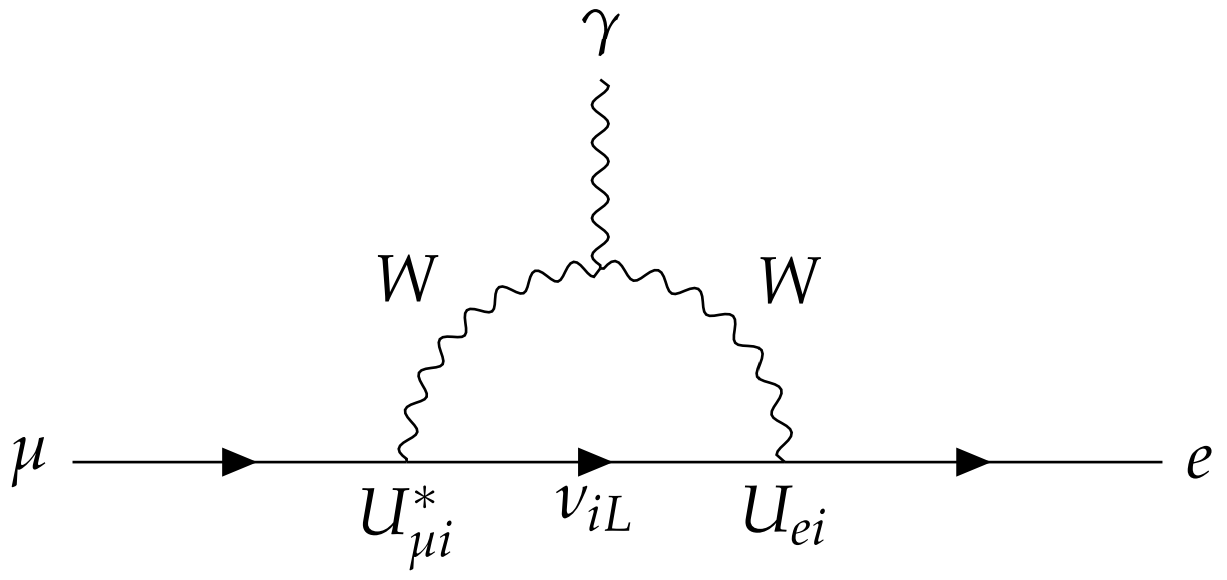
\includegraphics[scale = 0.2]{figures/png/Screenshot_20240217_171058.png}
         \subcaption{$\mu \rightarrow e \gamma$ process, Ref. \cite{universe8060299}.}
         \label{fig:mutoegamma}
     \end{subfigure}
     \begin{subfigure}[b]{0.7\linewidth}
         \centering
         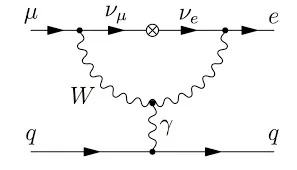
\includegraphics[scale = 0.5]{figures/jpg/1_erkKoywyuFzJmMv4PKpc9Q.jpg}
         \subcaption{$\mu N \rightarrow e N$ process.}
         \label{fig:mutoeN}
     \end{subfigure}
     \caption{Some of CLFV processes.}
        \label{fig:three graphs2}
\end{figure}
In the SM, each of these mechanisms is significantly inhibited. Using the example of $\mu \rightarrow  e \gamma $, the branching ratio (BR) of this process may be computed as follows:

\begin{equation}\label{br}
\begin{aligned}
B R(\mu \rightarrow e \gamma) & =\frac{3 \alpha}{32 \pi}\left|\sum_{i=2,3} U_{\mu i}^* U_{e i} \frac{\Delta m_{1 i}^2}{M_W^2}\right|^2 \\
& =\frac{3 \alpha}{32 \pi}\left(\frac{1}{4}\right) \sin ^2 2 \theta_{13} \sin ^2 \theta_{23}\left|\frac{\Delta m_{13}^2}{M_W^2}\right|^2,
\end{aligned}
\end{equation}

where $\alpha$ is the fine structure constant, $U_{\mu i}$ and $U_{ei}$ are corresponding elements in the PMNS matrix, $\Delta m_{1i}^2$ is the neutrino squared mass differences, $M_W$ is the $W$ boson mass and $\theta_{13}$ and $\theta_{23}$ are rotating angles in PMNS matrix parametrization. The expression yields $B R(\mu \rightarrow e \gamma) \sim \mathcal{O}(10^{-54})$. The big discrepancy in mass between neutrinos and the $W$ boson results in an extraordinarily small value for $|\Delta m_{13}^2/M_W|$. Equivalent suppression mechanisms are evident in other CLFV processes. The rates predicted by the Standard Model are extremely small, making them impractical for detection in any experiment. On the other hand, numerous Beyond the Standard Model (BSM) theories incorporate mechanisms that substantially amplify CLFV rates, a topic to be addressed in the subsequent section. The small value of SM CLFV rates implies that the detection of any CLFV processes in experiments would unequivocally indicate the presence of physics beyond the SM.
\subsection{Beyond the Standard Model}
Numerous Beyond the Standard Model (BSM) theories propose mechanisms that could contribute to CLFV processes, potentially yielding detectable rates in experiments. Here, we highlight a selection of BSM theories known for their CLFV contributions. It is important to note that this list is not comprehensive; for further studies, additional reviews are available in Ref. \cite{clfv_signorelli} and Ref. \cite{universe8060299}.
\subsubsection{CLFV in Supersymmetry}\label{susy}
Supersymmetry (SUSY) is a theoretical framework that has oriented experiments in the CLFV reasearch for many years. On one hand, models with SUSY broken at energies close to electro-weak scale have given solution to the hierarchy problem, i.e. how to maintain the Higgs mass significantly smaller than the Planck scale ($\sim$10$^{19}$ GeV). On the other hand, the suppression of CLFV processes is due to the wide separation of the neutrinos and $W$ masses, which can be mitigated by introducing SUSY partners of neutrinos and $W$ bosons. This suggests that CLFV processes should have been observable earlier, unless SUSY breaking occurs at or near the electroweak scale ($\sim 10^2$ GeV), Ref. \cite{clfv_signorelli}. In this framework, each elementary particle has a superpartner,  with the same quantum numbers except for spin: a boson is the superpartner of a fermion and vice versa. A superpartner of a lepton is called $slepton$. If there is no common eigenstate base between lepton and $slepton$'s mass matrices then a physical $slepton$ will be a superposition of flavors. In this case a loop diagram can lead to CLFV, as shown in Fig.\ref{fig:susy}. Despite the similar topology to that of the SM contribution (Fig.\ref{fig:mutoegamma}), the typical SUSY mass is expected to be much higher than that of the neutrinos. Predictions for the branching ratio of this process vary among different SUSY models, contingent upon specific mechanisms and particle masses. These rates can undergo significant enhancement. For example, in an $SU(5)$ SUSY grand unified theory, the computed branching ratio could reach $\mathcal{O}(10^{-14})$ for a slepton mass on the order of $\mathcal{O}(10^{-14}$ GeV/c$^2)$, a value measurable for upcoming experiments.

\begin{figure}[!h]
\centering
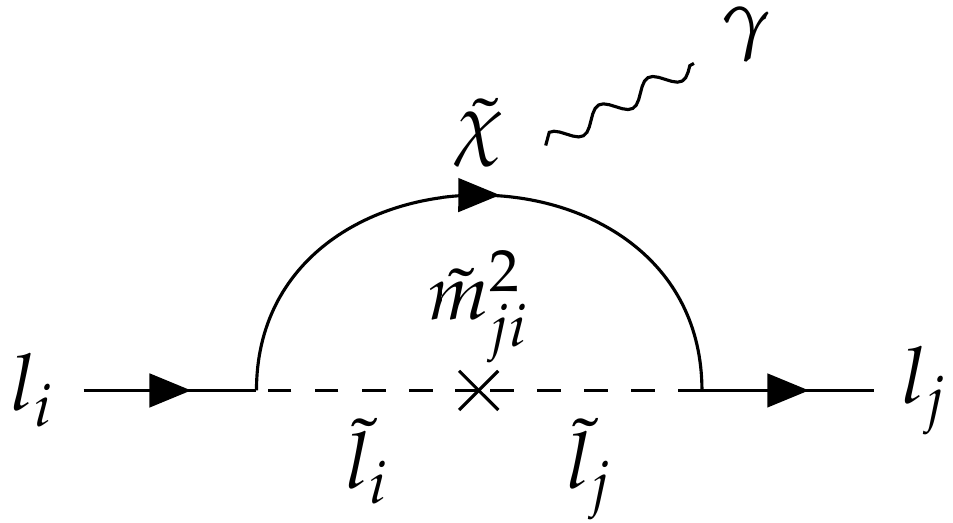
\includegraphics[width =0.4\textwidth]{figures/png/Screenshot_20240218_105920.png}
\caption{SUSY contribution to $l_i \rightarrow l_j\gamma$, through $sleptons$ mass mixing, Ref. \cite{universe8060299}.}
\label{fig:susy}
\end{figure}


\subsubsection{Two Higgs Doublet Model}\label{2higgs}
Although the Standard Model (SM) incorporates only one Higgs boson, there are no constraints against the presence of additional Higgs fields. One straightforward example of a comprehensive theory featuring multiple Higgs fields is the type III two Higgs doublet model (2HDM), where two Higgs bosons exist, each interacting with fermions and possessing a vacuum expectation value, Ref. \cite{Harnik_2013}. Generally, the Lagrangian incorporating extra Higgs fields post-electroweak symmetry breaking can be written as:
\begin{equation}
-\mathscr{L}=m_i \bar{f}_{L i} f_{R i}+\left(Y^\alpha\right)_{i j} \bar{f}_{L i} f_R{ }_j h^\alpha+\text { h.c. }+\ldots
\end{equation}
Non renormalizable terms of higher dimensions are omitted. $(Y^\alpha)_{i j}$ represents couplings to a single scalar field and the contributions from different Higgses are summed over. The non-zero-off-diagonal terms in $(Y^\alpha)_{i j}$ give rise to flavor violating Yukawa couplings. From accelerator and precision experiments, constraints on the off-diagonal coupling of the 125 GeV Higgs boson can be obtained.
\subsubsection{Leptoquark Models}
Leptoquarks (LQs) are theoretical particles initially proposed within the Pati-Salam model, Ref. \cite{PhysRevD.10.275}. Each LQ is linked to both baryon number ($B$) and lepton number ($L$). In various LQ models the quark and lepton sectors are unified. This unification allows for direct coupling between quarks and leptons via the exchange of LQs. Consequently, specific CLFV processes like $K_L^0 \rightarrow e \mu$ and $\mu N \rightarrow e N$ are mediated by LQs. Constraints on LQ models arise from both collider experiments and rare decay searches. Direct searches at ATLAS and CMS have excluded scalar LQs of the first and second generations with masses below $\sim$1 TeV. Indirect searches provide constraints on the mass-coupling plane, where regions with higher couplings and lower LQ masses correspond to higher branching ratios. Additionally, LQ models must satisfy constraints related to proton stability, as some models involve LQs that could mediate proton decay. To mitigate this, the corresponding LQs must either have extremely high masses or their related couplings must be exceedingly small, Ref. \cite{DORSNER20161}.
\subsubsection{Additional Neutral Gauge Boson}
Grand unified theories (GUTs) are constructed based on extended gauge groups in the pursuit of a more fundamental model. At lower energies, these extended gauge groups are believed to break down to the direct product of the Standard Model (SM) gauge group $SU(3) \times SU(2) \times U(1)$ along with an additional $U(1)$ factor. The neutral gauge boson associated with this $U(1)$ group can mix with the original SM neutral gauge boson, resulting in two mass eigenstates, namely $Z$ and $Z'$. Additionally, extended gauge theories require the introduction of additional fermion fields to cancel anomaly-free currents beyond those of $SU(5)$. These $new$ fermions can mix with the known SM fermions possessing the same electric and color charges, consequently affecting their couplings with gauge bosons. The appearance of off-diagonal terms in neutral current couplings to fermions can lead to flavor-changing couplings to $Z$ and $Z'$. Certain CLFV processes, such as $\mu \rightarrow eee$ and $\mu-e$ conversion, receive tree-level contributions through intermediate $Z$ and $Z'$ bosons. Further insights into the phenomenology of the $Z'$ boson can be found in, Ref. \cite{Leike_1999}. The search for the existence of $Z'$ bosons is conducted through channels like $Z' \rightarrow \bar{f}f$ at hadron colliders. Mass lower limits of $Z'$ from various specific models are listed in Ref. \cite{zyla}, primarily falling within the low TeV range. Particularly, mass lower limits reported in CLFV final states $e\mu$, $e\tau$ and $\mu\tau$ range between 3.5 TeV and 4.5 TeV. Upper limits of $Z \rightarrow l_1 l_2$ couplings to the normal Z boson are also provided in Table \ref{tab:upperlimits}.
%Quello che segue è un esempio di codice. E' possibile modificare il linguaggio per il synyax highlight, aggiungere parole chiave... E' tutto disponibile nella guida del pacchetto \texttt{listings}.

%\lstinputlisting[language=C++]{listings/png/code1.cpp} 
\section{Experiments looking for CLFV}
Charged Lepton Flavor Violation has not been observed yet, despite ongoing efforts to detect such violations across various channels in both dedicated and general-purpose experiments. Some of these efforts are documented in Table \ref{tab:upperlimits}, which presents their respective experimental upper limits.
\begin{center}  
\begin{table}[!h]
\centering
\renewcommand{\arraystretch}{1.5}
\begin{tabular}{c c c c c c}
\hline
Reaction & Present limit & C.L. & Experiment &  Year & Ref.\\
\hline
$\mu^+\ \rightarrow \ e^+ \ \gamma$& $7.5 \times 10^{-13}$ & 90\% & MEG II & 2024 & \cite{megiicollaboration2024search}\\
$\mu^+ \ \rightarrow \ e^+ \ e^+ \ e^-$ & $1.0 \times 10^{-12}$ & 90\% & SINDRUM & 1988 & \cite{SINDRUM:1987nra} \\
$\mu^- \ \text{Ti}\ \rightarrow \ e^- \ \text{Ti}$ &  $6.1 \times 10^{-13}$ & 90\% & SINDRUM II & 1998 & \cite{titanium}\\
$\mu^- \ \text{Au}\ \rightarrow \ e^- \ \text{Au}$ & $7.0 \times 10^{-13}$ & 90\% & SINDRUM II & 2006 & \cite{SINDRUMII:2006dvw} \\
$\mu^+ \ e^- \ \rightarrow \ \mu^- \ e^+$ & $8.3 \times 10^{-11}$ & 90\% & SINDRUM & 1999 & \cite{Willmann:1998gd}\\
$\tau \ \rightarrow \ e \ \gamma$ & $3.3 \times 10^{-8}$ & 90\% & BaBar & 2010 & \cite{Aubert_2010}\\
$\tau \ \rightarrow \ \mu \ \gamma$ & $4.4 \times 10^{-8}$ & 90\% & BaBar & 2010 & \cite{Aubert_2010}\\
$\tau \ \rightarrow \ e \ e \  e$ & $2.7 \times 10^{-8}$ & 90\% & Belle & 2010 & \cite{Hayasaka_2010}\\
$\tau \ \rightarrow \ \mu \ \mu  \ \mu$ & $2.1 \times 10^{-8}$ & 90\% & Belle & 2010 & \cite{Hayasaka_2010} \\
$B^0 \ \rightarrow \ \mu \ e$ & $2.8 \times 10^{-9}$ & 90\% & LHCb & 2013 & \cite{PhysRevLett.111.141801}\\
$B^0 \ \rightarrow \ \tau \ e$ & $2.8 \times 10^{-5}$ & 90\% & BaBar & 2008 & \cite{PhysRevD.77.091104}\\
$B^0 \ \rightarrow \ \tau \ \mu$ & $2.2 \times 10^{-5}$ & 90\% & BaBar & 2008 & \cite{PhysRevD.77.091104}\\
$K_L^0 \ \rightarrow \ \mu \ e$ & $4.7 \times 10^{-12}$& 90\% & BNL E871 & 1998 & \cite{BNL:1998apv}\\
$K^+\ \rightarrow \ \pi^+ \ \mu^+ \ e^-$ & $2.1 \times 10^{-10} $ & 90\% & BNL E865 & 2005 & \cite{PhysRevD.72.012005}\\
$K_L^0 \ \rightarrow \ \pi^0 \ \mu^+ \ e^-$ & $ 4.4 \times 10^{-10}$ & 90\% & KTeV & 2008 & \cite{KTeV:2007cvy}\\
$Z^0 \ \rightarrow \ \mu \ e$ & $1.7 \times 10^{-6}$ & 95\% &  LHC ATLAS & 2014 & \cite{Aad_2014} \\
$Z^0 \ \rightarrow \ \tau \ e$ & $1.7 \times 10^{-6}$ & 95\% &  LEP OPAL & 1995 & \cite{akers}\\
$Z^0 \ \rightarrow \ \tau \ \mu$ & $9.8 \times 10^{-6}$ & 95\% &  LEP DELPHI & 1997 & \cite{abreu}\\
$\pi^0 \ \rightarrow \ \mu \ e$ & $8.6 \times 10^{-9}$ & 90\% & KTeV & 2008 & \cite{KTeV:2007cvy}\\
$\Upsilon (1s) \ \rightarrow \ \mu \ \tau $ & $6.0 \times 10^{-6}$ & 95\% & CLEO & 2008 & \cite{Love_2008}\\
\hline
\end{tabular}
\caption{Experimental upper limits for a variety of CLFV processes, Ref. \cite{clfv_signorelli}.}
\end{table}\label{tab:upperlimits}
\end{center}


\subsection{$\mu$ Channels}
Currently, the most promising channel is the one that includes muon processes. When a proton beam interacts with a target, pions and kaons are produced, that subsequently decay in muons. Muon lifetime is long enough to form a muon beam and we are able to reach intensities of 10$^8 \div 10^{11} \  \mu$/s. There are three primary CLFV channels involving muons, with distinct sensitivities to effective lagrangian terms: $\mu^+ \rightarrow e^+ \gamma$, $\mu^- N \rightarrow e^- N$ and $\mu^+ \rightarrow e^+ e^+ e^-$. The following paragraphs will discuss the experimental challenges and future perspectives for each of these channels. As seen in Table \ref{tab:upperlimits}, these channels have the lowest branching ratio limits. Muons have small mass, that results in a limited number of decay modes. Figure \ref{fig:muchannel} shows how the branching ratio limitations of muon uncommon decays have rapidly improved over the last several decades. The next-generation experiments aim to improve by many orders of magnitude. Muon rare decay studies can also provide theory differentiation power combining results of the three channels. All CLFV extensions to SM can be described by the following Lagrangian, Ref. \cite{doi:10.1146/annurev-nucl-100809-131949}:
\begin{equation}\label{LCF}
\mathscr{L}_{C L F V}=\frac{m_\mu}{(1+\kappa) \Lambda^2} \bar{\mu}_R \sigma_{\mu \nu} e_L F^{\mu \nu}+\text{h.c.}+\frac{\kappa}{(1+\kappa) \Lambda^2} \bar{\mu}_L \gamma_\mu e_L\left(\sum_{q=u, d} \bar{q}_L \gamma^\mu \bar{q}_L\right)+\text{h.c.}
\end{equation}
$m_\mu$ is the muon mass and  $F^{\mu \nu}$ is the electromagnetic field tensor. This toy Lagrangian includes two parameters.
$\Gamma$ is the effective energy scale of the new physics and $\kappa$ is the relative strengths of the two operators. The first term in the Lagrangian 
is a magnetic-moment-type operator and describes all three processes mentioned above, it is generated by any loop with some new particle that can be either virtual and real.
The second one corresponds to a four-fermion operator, which mediates $\mu N \rightarrow eN$ at tree level and the other two processes at one-loop level.
The Mu2e experiment can probe an effective mass scale up to $\mathcal{O}$(10$^4$ TeV) with its designed sensitivity assuming $\kappa$ $\gg$ 1.
On the other hand, $\mu \rightarrow e\gamma$ experiments are more sensitive when $\kappa$ $\ll$ 1; the dominant magnetic
moment type term determines the other two processes have lower rates in such a case. In order to learn more about the new
physics, one needs to combine information involving the rates of a different CLFV processes, Ref. \cite{osti_1042577}.
The corresponding parameter space (the $\Gamma-\kappa$ plane) is shown in Figure \ref{fig:muchannelbr}, Ref. \cite{doi:10.1146/annurev-nucl-100809-131949}.
\begin{figure}[!h]
\centering
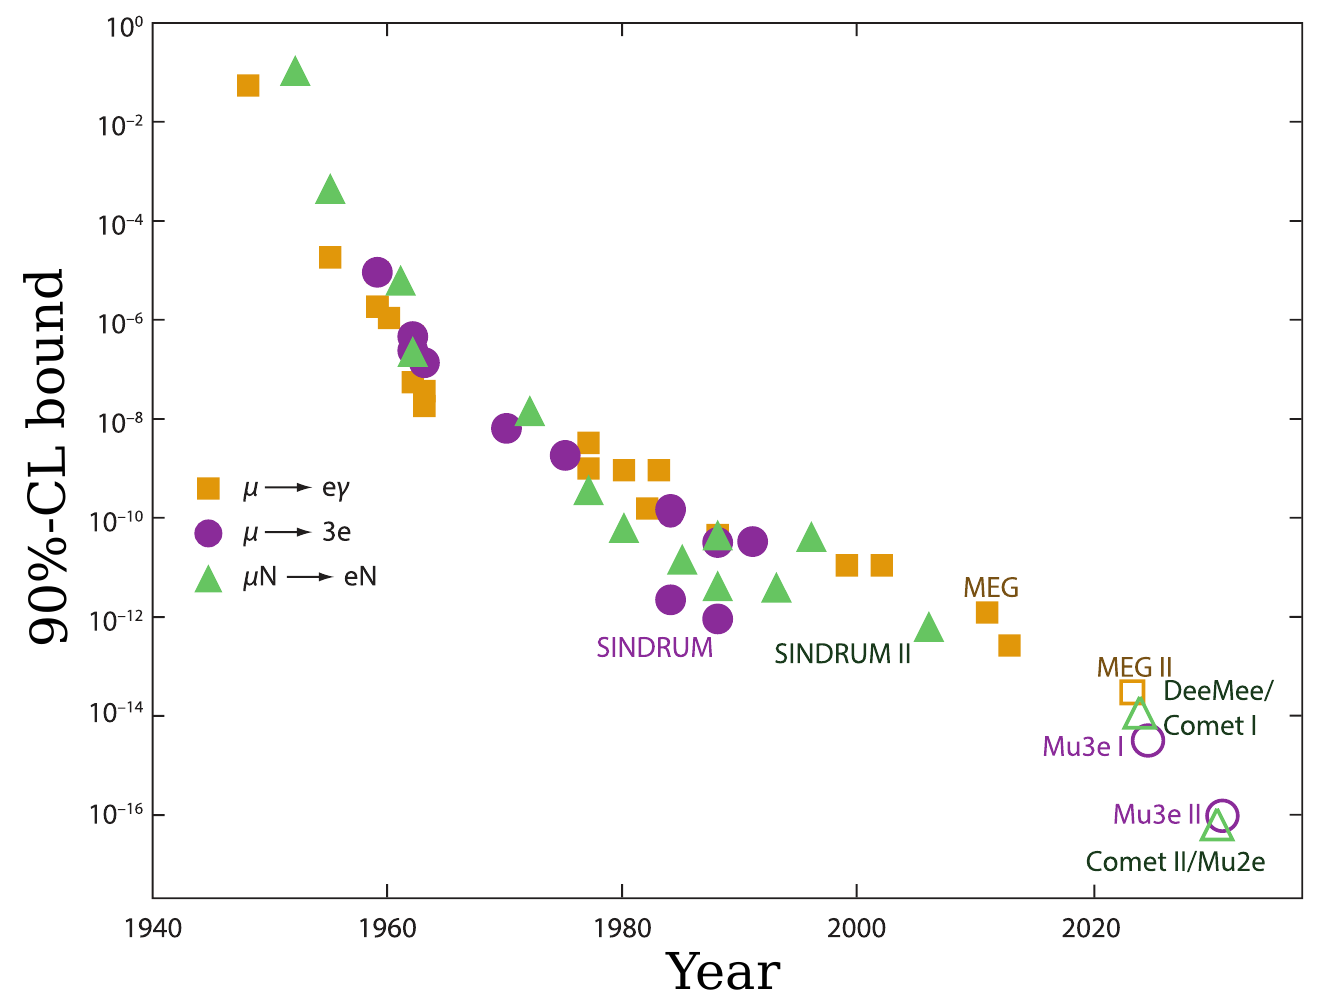
\includegraphics[width =0.8\textwidth]{figures/png/Screenshot_20240307_161549.png}
\caption{History and outlook of branching ratio limits in muon rare decay modes, Ref. \cite{MARCIANO1977303}.}
\label{fig:muchannel}
\end{figure}
\begin{figure}[!h]
\centering
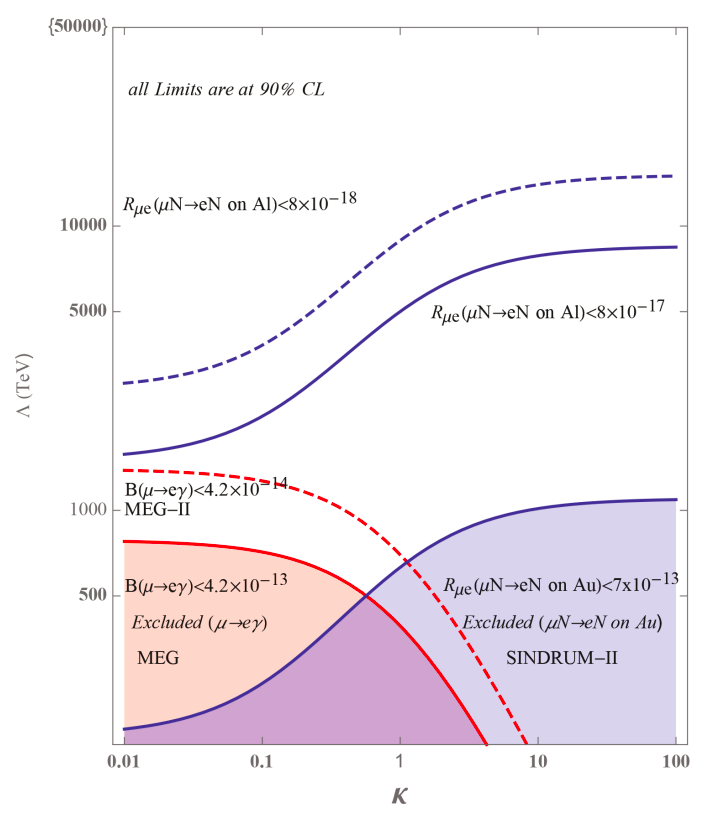
\includegraphics[width =0.8\textwidth]{figures/png/Screenshot_20240313_120457.png}
\caption{Sensitivity of $\mu \rightarrow e\gamma$ and $\mu N \rightarrow eN$ experiments to the new physics
scale $\Gamma$ as a function of $\kappa$ as defined in Equation \ref{LCF}, Ref. \cite{CGroup:2022tli}. The blue region is the New
Physics phase space excluded by SINDRUM-II, Ref. \cite{SINDRUMII:2006dvw}. The red region represents the
limit set by MEG, Ref. \cite{megi}, while the dashed red line represents the region that is
excluded by MEG-II, Ref. \cite{megiicollaboration2024search}. The solid (dashed) blu line is the
expected limit that would be set by Mu2e, Ref. \cite{universe9010054}.}
\label{fig:muchannelbr}
\end{figure}
\subsubsection{$\mu^+ \rightarrow e^+ \gamma$}
\paragraph{The MEG Experiment}
\cite{megi}
\begin{figure}[!h]
\centering
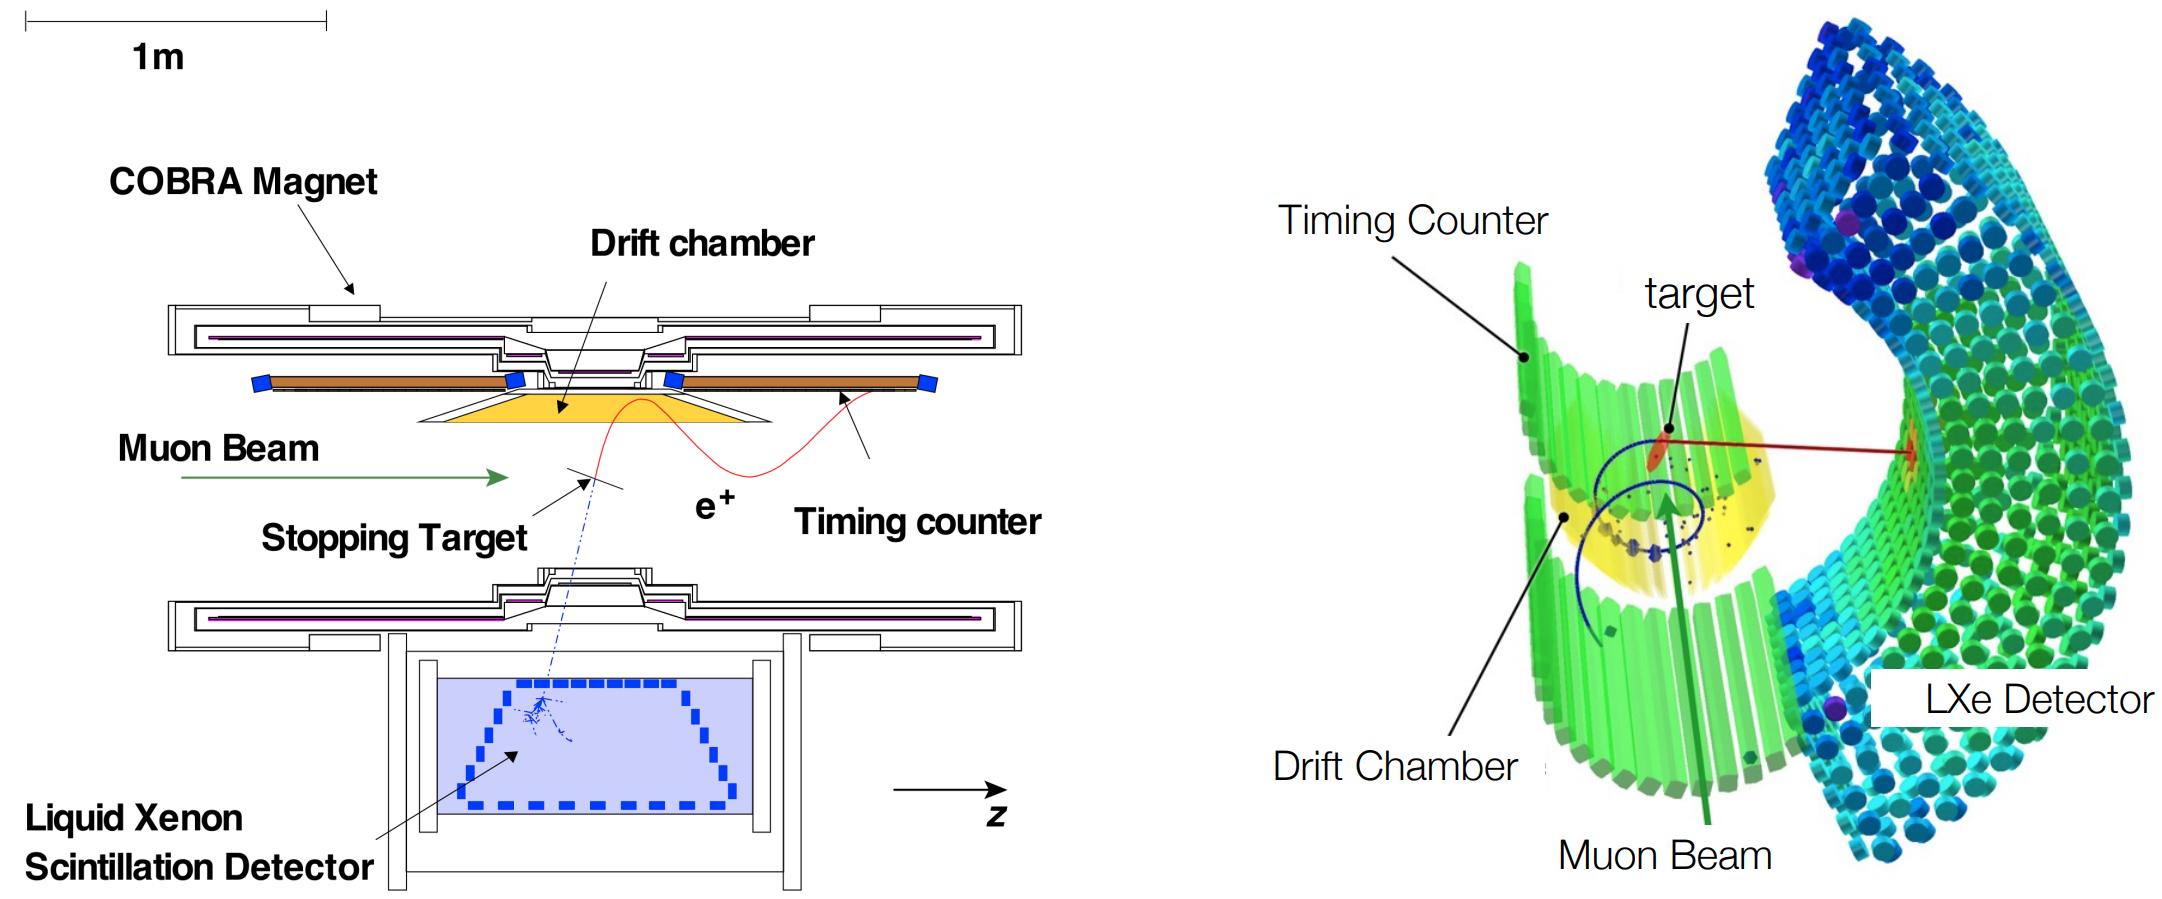
\includegraphics[width =0.4\textwidth]{figures/png/Screenshot_20240307_150038.png}
\caption{.}
\label{fig:meg}
\end{figure}
\paragraph{MEG II}
\cite{megiicollaboration2024operation}
\cite{megiicollaboration2024search}
\begin{figure}[!h]
\centering
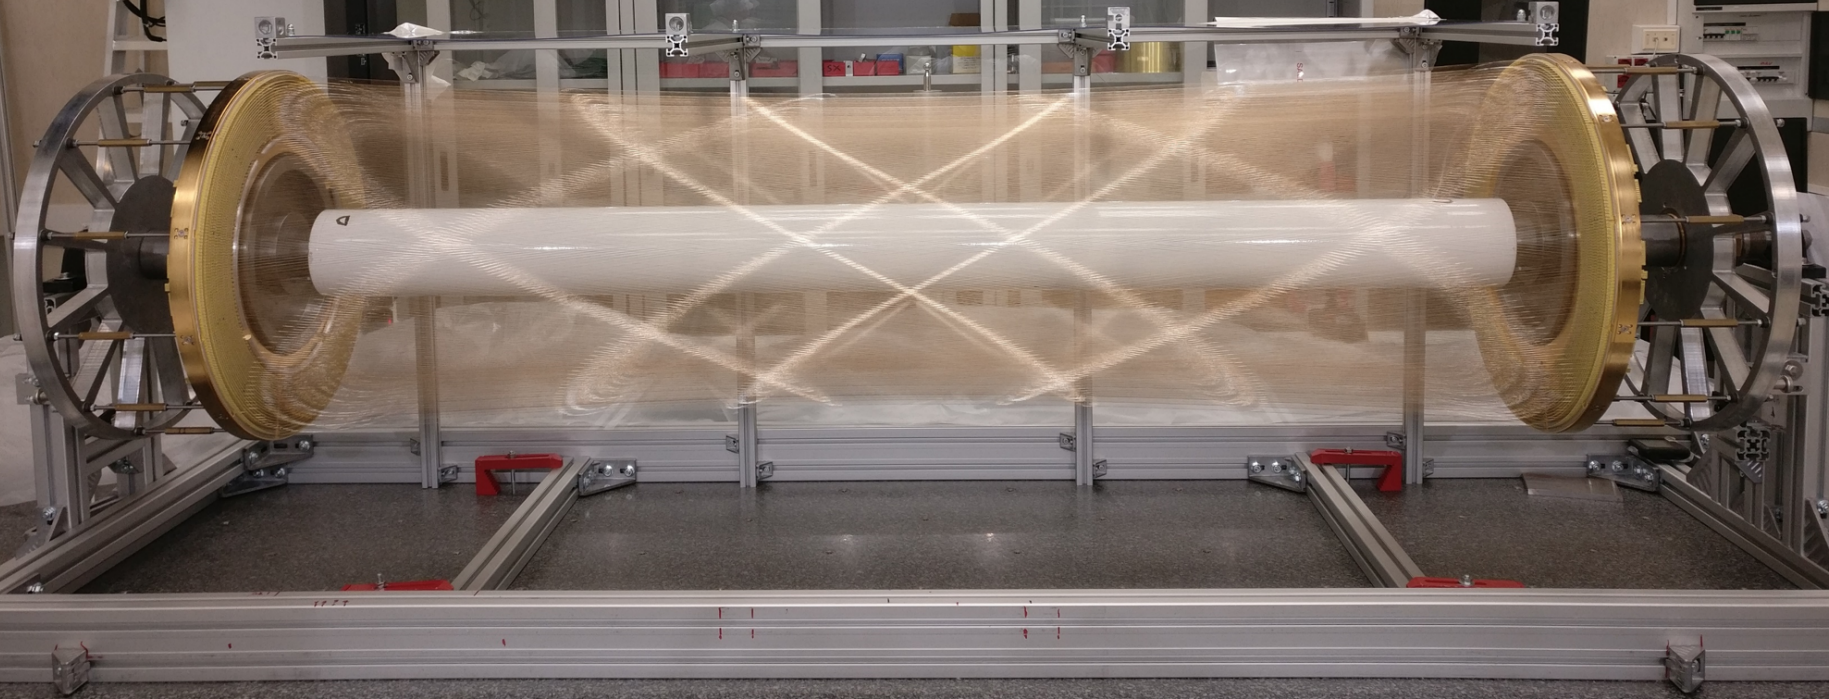
\includegraphics[width =0.4\textwidth]{figures/png/Screenshot_20240307_140235.png}
\caption{.}
\label{fig:meg2}
\end{figure}
\begin{figure}[!h]
\centering
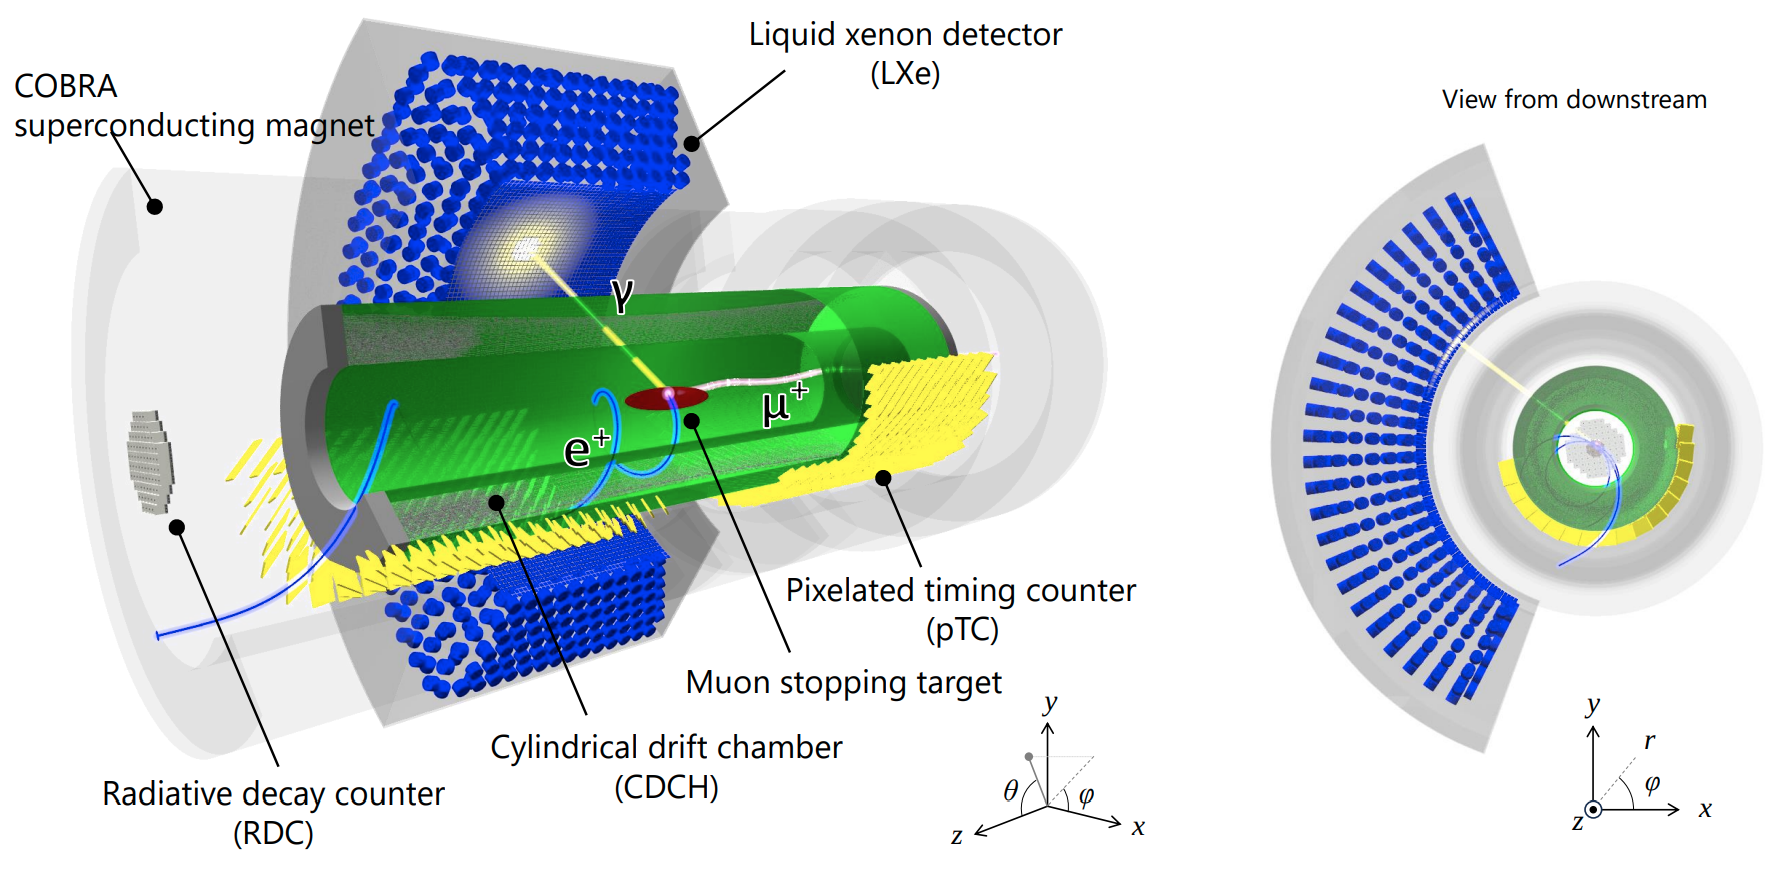
\includegraphics[width =0.4\textwidth]{figures/png/Screenshot_20240307_140116.png}
\caption{.}
\label{fig:meg22}
\end{figure}
\subsubsection{$\mu^+ \rightarrow e^+ e^-  e^+ $}
\paragraph{SINDRUM I}
\cite{sindrumi}
\begin{figure}[!h]
\centering
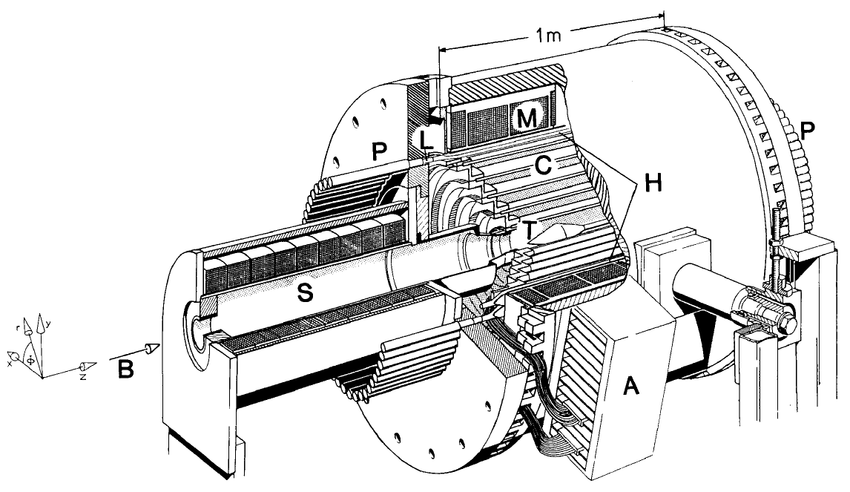
\includegraphics[width =0.4\textwidth]{figures/png/The-SINDRUM-I-detector-in-the-horizontal-operating-orientation.png}
\caption{.}
\label{fig:sindrumi}
\end{figure}
\paragraph{The Mu3e Experiment}

\begin{figure}[!h]
\centering
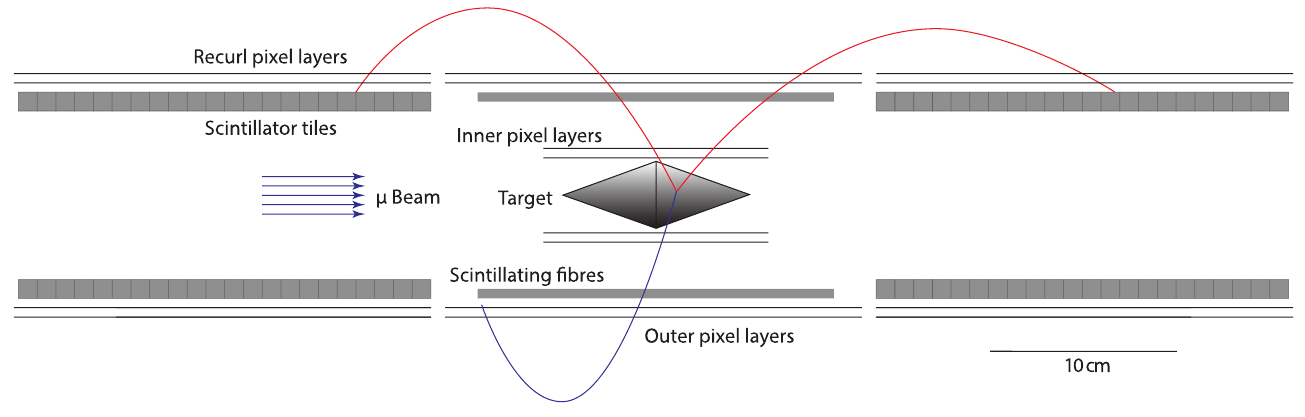
\includegraphics[width =0.4\textwidth]{figures/png/Screenshot_20240307_161651.png}
\caption{Longitudinal cross section of the detector. Positrons tracks in red, electron
track in blue \cite{hesketh2022mu3e}}
\label{fig:mu3e}
\end{figure}
\subsubsection{$\mu^- N \rightarrow e^- N $}
\paragraph{SINDRUM II}
\cite{SINDRUMII:2006dvw}
\begin{figure}[!h]
\centering
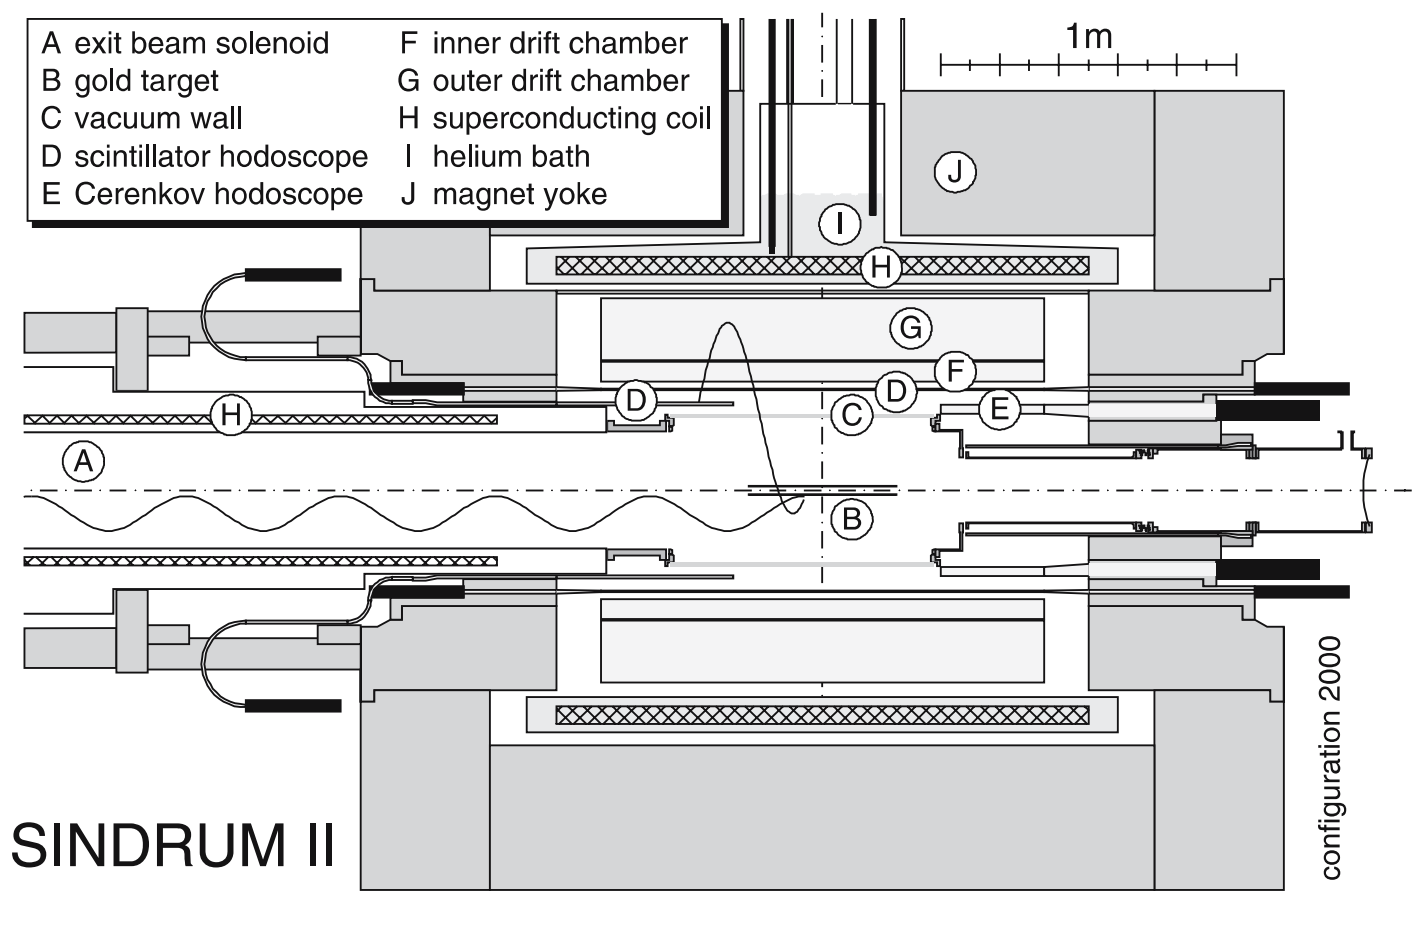
\includegraphics[width =0.4\textwidth]{figures/png/Screenshot_20240307_163120.png}
\caption{.}
\label{fig:sindrumii}
\end{figure}
\paragraph{Mu2e}
\paragraph{COMET}
\cite{Abramishvili_2020}
\begin{figure}[!h]
\centering
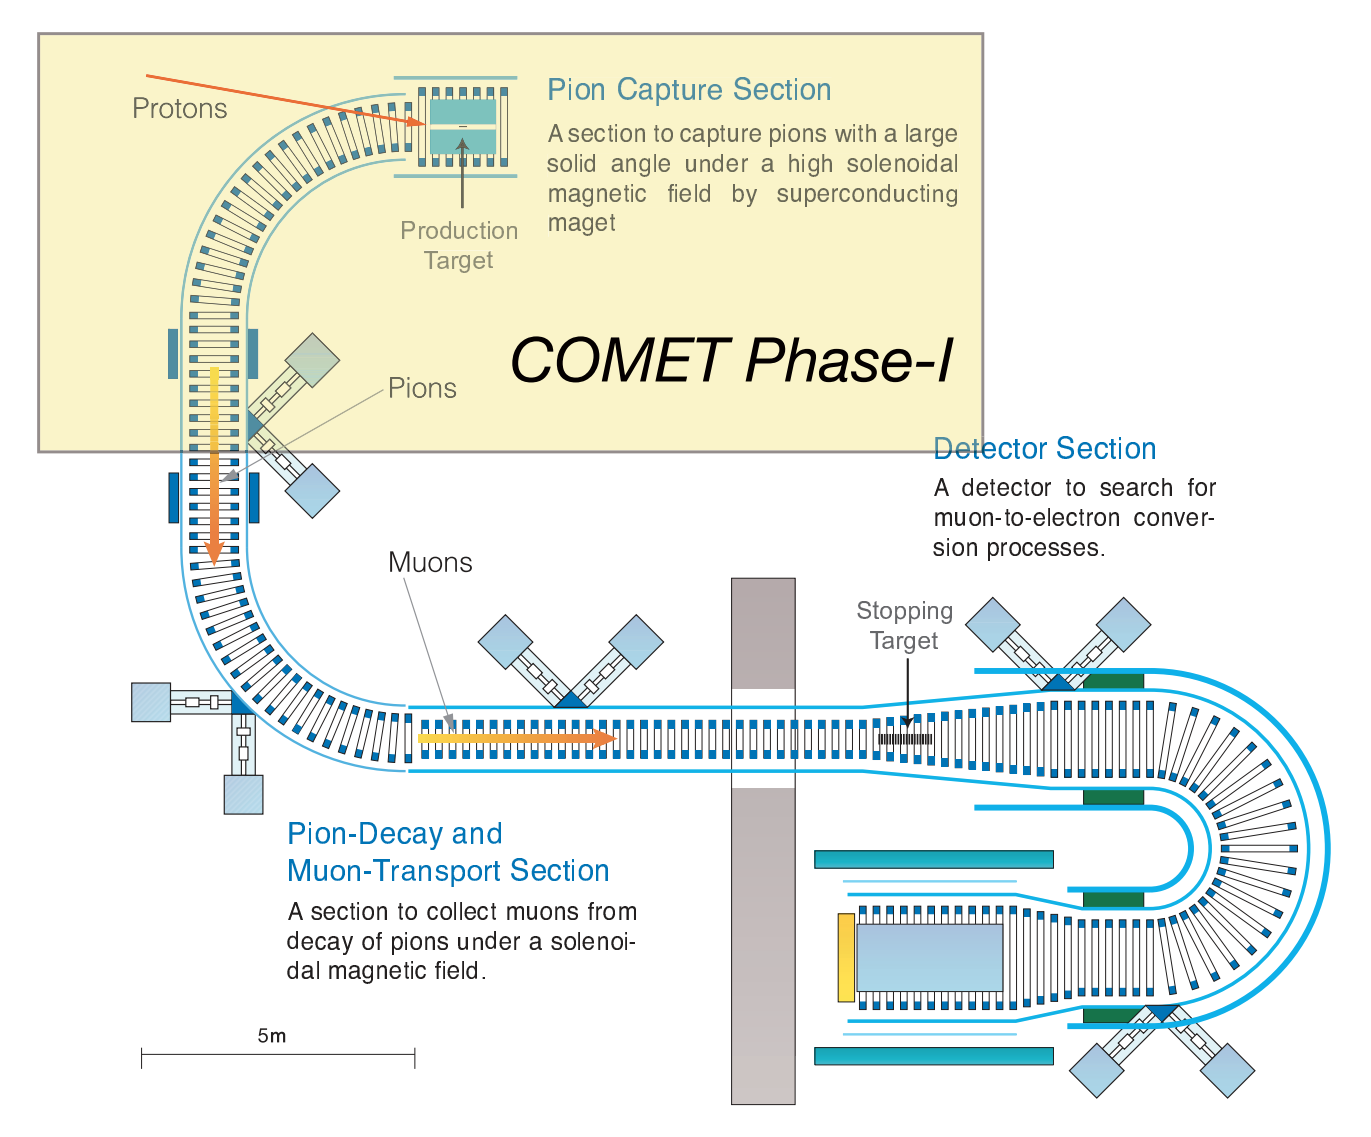
\includegraphics[width =0.4\textwidth]{figures/png/Screenshot_20240307_152133.png}
\caption{Schematic layout of COMET (Phase-II) and COMET Phase-I (not in scale).}
\label{fig:comet}
\end{figure}
\paragraph{Mu2e II}
\cite{dukes}
\subsection{$\tau$ Channels}
The tau lepton is a very promising source of CLFV decays, Ref. \cite{universe8060299}. 
The huge tau mass ($m_\tau$ $\sim$ 1.777 GeV) allows for the investigation of multiple CLFV channels: 
$\tau^\pm \rightarrow \mu^\pm \gamma$, $\tau^\pm \rightarrow e^\pm \gamma$, $\tau \rightarrow 3l$ and $\tau\rightarrow l \ h$, 
where $h$ is a light hadron and $l$ is an electron or muon. The $\tau$ sector of a CLFV search takes advantage from an higher predicted branching ratio, compared to muons according 
to equation \ref{br}. Table \ref{tab:upperlimits} lists the current best limits on the $\tau$ CLFV searches and Figure \ref{fig:tauchannel} displays the results from the BaBar, 
Ref. \cite{PhysRevD.77.091104}, Belle, Ref. \cite{ABASHIAN2002117} and LHCb, Ref. \cite{TheLHCbCollaboration2008} experiments.
The $\tau$ is unstable and has a relatively short lifetime ($\tau_\tau \ \sim$ 2.91 $\times$ 10$^{-13}$ s).
As a result, it is not possible to produce $\tau$ beams and strong electron or proton accelerators are required to produce $\tau$s with a large generation cross section. 
At $e^+ e^-$ and $pp$ collider machines, the $\tau$s are not created at rest: it is necessary to deal with decays-in-flight. 
Because of the boost, the decay products could have energy of several GeV, posing the experimental challenge of providing wide-range calibrations for detectors 
(from a few hundred MeV to several GeV), Ref. \cite{universe8060299}. In these experiments, a pair of $\tau^+ \tau^-$ will be produced by the decay of 

For each of these searches, events include a $\tau$ pair wherein one $\tau$ decays via Standard Model (SM) process (tag side), 
while the signal side is determined based on the specific topology of each channel. 
The tag side accommodates leptonic ($\tau$ $\rightarrow$ $l \nu\bar{\nu}$) and 1-prong hadronic decays, whereas on the signal side, 
candidates for Charged Lepton Flavor Violation (CLFV) are chosen according to the appropriate topology of each channel. Subsequent sections delve into the latest constraints achieved in some of these experimental quests conducted at $B$-factories and $pp$ colliders, as documented in Ref. \cite{universe8060299}.
\begin{figure}[!h]
\centering
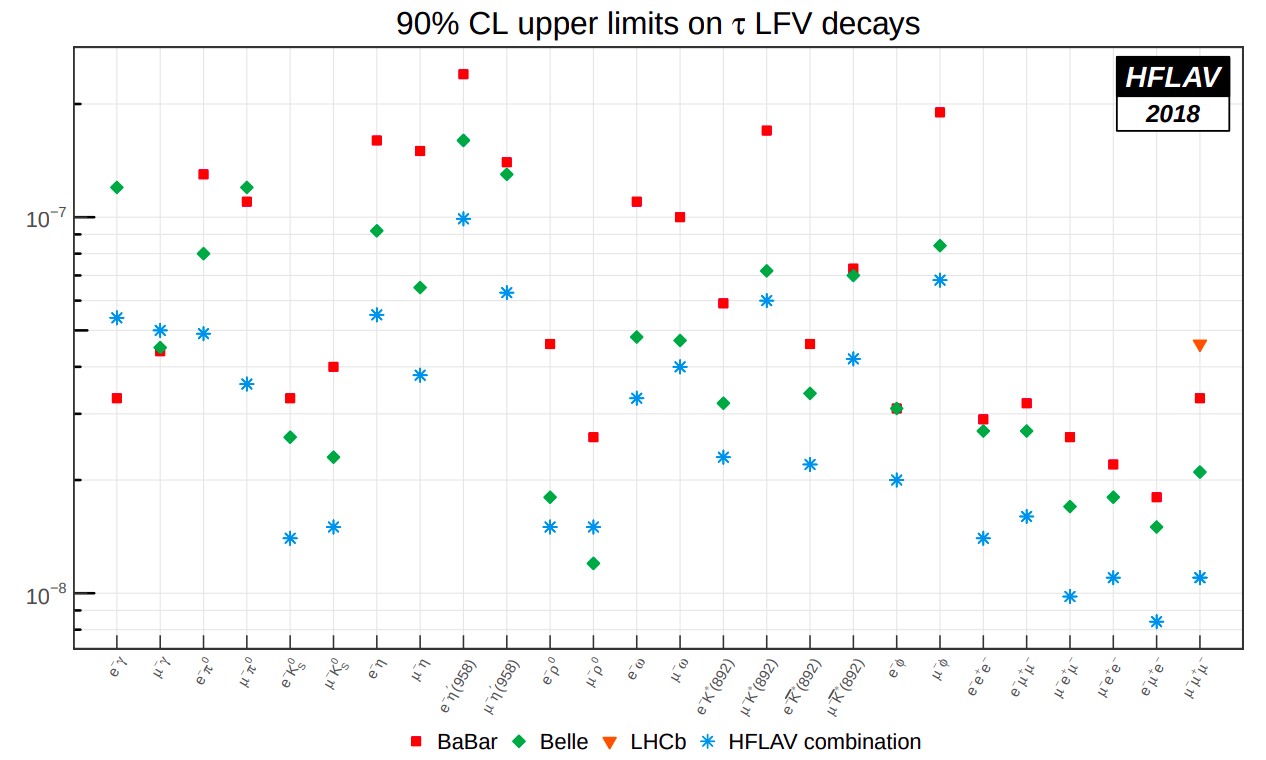
\includegraphics[width =0.4\textwidth]{figures/png/Screenshot_20240313_133439.png}
\caption{\cite{Amhis_2021}.}
\label{fig:tauchannel}
\end{figure}
\subsubsection{$ \tau \rightarrow l \gamma$}
\iffalse
The $\tau \rightarrow l\gamma$ decay, where $l$ is a light lepton $(e, \mu)$, has been one of the most popular
CLFV tau channels. The signal is characterized by a $l^\pm - \gamma$ pair with an invariant mass
and total energy in the center-of-mass (CM) frame (ECM) close to mτ = 1.777 GeV and
√
s/2, respectively. The dominant irreducible background comes from τ-pair events containing hard photon radiation and one of the τ leptons decaying to a charged lepton. The
remaining backgrounds arise from the relevant radiative processes, e
+e
− → e
+e
−γ and
e
+e
− → µ
+µ
−γ and from hadronic τ decays where a pion is misidentified as an electron
or muon. For this decay channel, the current best limits comes from the BaBar and the
Belle collaborations. BaBar collected (963 ± 7) × 106 τ decays near the Υ(4S), Υ(3S) and
Υ(2S) resonances. In the BaBar detector [179], charged particles are reconstructed as tracks
with a 5-layer silicon vertex tracker and a 40-layer drift chamber inside a 1.5 T solenoidal
magnet. A CsI(Tl) electromagnetic calorimeter is used to identify electrons and photons. A
ring-imaging Cherenkov detector is used to identify charged pions and kaons. The flux
return of the solenoid, instrumented with resistive plate chambers and limited streamer
tubes, is used to identify muons. Signal decays are identified by two kinematic variables:
the energy difference ∆E = ECM −
√
s/2 and the beam energy constrained τ mass obtained
from a kinematic fit after requiring the CM τ energy to be √
s/2 and after assigning the
origin of the γ candidate to the point of closest approach of the signal lepton track to the
e
+e
− collision axis (mBC). Figure 21 shows the distributions of the events for the two decay
channels in mBC vs. ∆E. The red dots are experimental points, the black ellipses are the 2σ
signal contours and the yellow and green regions contain 90\% and 50\% of MC signal events. The searches yield no evidence of signals, and the experiment set upper limits on the
branching fractions of B(τ
± → e
±γ) < 3.3 × 10−8 and B(τ
± → µ
±γ) < 4.4 × 10−8 at 90%
confidence level [140].
The Belle experiment [180] reported comparable limits using a data analysis based
on 988 fb−1
and a strategy similar to that of BaBar. Kinematical selections on missing
momentum and opening angle between particles are used to clean the sample. Figure 22
shows the two-dimensional distribution of∆E/
√
s vs. mBC. The signal events have mBC ∼
mτ and ∆E/
√
s ∼ 0. The most dominant background in the τ
± → µ
±γ (τ± → e
±γ )
search arises from τ
+τ
− events decaying to τ
± → µ
±νµντ (τ
± → e
±νeντ) with a photon
coming from initial-state radiation or beam background. The µ
+µ
−γ and e
+e
−γ events
are subdominant, with their contributions falling below 5\%. Other backgrounds such as
two-photon and e
+e
− → qq¯ (q = u, d, s, c) are negligible in the signal region
No significant excess over background predictions from the Standard Model is observed, and the 90% C.L. upper limits on the branching fractions are set at B(τ
± → µ
±γ) ≤
4.2 × 10−8 and B(τ
± → e
±γ) ≤ 5.6 × 10−8
[183]. With the full dataset expected for the
Belle II experiment [184] (the upgrade of Belle), 50 ab−1
, the upper limit for the branching
fraction of LFV decays τ will be reduced by two orders of magnitude
\fi
\subsubsection{$ \tau \rightarrow 3l $}
\iffalse
The signature for τ → 3l (l = e, µ) is a set of three charged particles, each identified
as either an e or a µ, with an invariant mass and energy equal to that of the parent τ lepton.
In the BaBar [185] and Belle [141] analyses, all the six different combinations were
explored. Events are preselected requiring four reconstructed tracks and zero net charge,
selecting only tracks pointing toward a common region consistent with τ
+τ
− production
and decay. The polar angles of all four tracks in the laboratory frame are required to
be within the calorimeter acceptance range, to ensure good particle identification. The
search strategy consists of forming all possible triplets of charged leptons with the required
total charge and of looking at the distribution of events in the (mBC , ∆E) plane (mBC and
∆E are defined as in the previous section). The backgrounds contaminating the sample
can be divided in three broad categories: low multiplicity e
+e
− → qq¯ (q = u, d, s, c)
events, QED events (Bhabha or µ
+µ
− depending on the specific channel) and SM τ
+τ
−
events. These background classes have distinctive distributions in the (mBC, ∆E) plane.
The e
+e
− → qq¯ (q = u, d, s, c) events tend to populate the plane uniformly, while
QED backgrounds fall in a narrow band at positive values of ∆E, and τ
+τ
− backgrounds
are restricted to negative values of both ∆E and mBC due to the presence of at least one
undetected neutrino. Figure 20 shows the resulting limit for all the combinations to be at
the level of a few 10−8
for both collaborations.
Even if the results are not yet competitive to those from B-factories, it is interesting
to note that experiments at the LHC have also been looking for the τ → 3µ decay. The
ATLAS experiment [186] performed a search for the neutrinoless decay τ
− → µ
−µ
+µ
−
using a sample of W− → τ
−ν¯τ decays from a dataset corresponding to an integrated
luminosity of 20.3 fb−1
collected in 2012 at a center-of-mass energy of 8 TeV. The LHCb
experiment [187] performed the same search using a sample of tau from b and c-hadron
decays from a dataset corresponding to an integrated luminosity of 3.0 fb−1
collected by
the LHCb detector in 2011 and 2012 at center-of-mass energies of 7 and 8 TeV, respectively.
The CMS experiment [188] recently delivered the results for the same search using a sample
of τ leptons produced in both W boson and heavy-flavour hadron decays from a dataset
corresponding to an integrated luminosity of 33.2 fb−1
recorded by the CMS experiment in
2016 [188]. ATLAS, CMS and LHCb reported a 90\% C.L. upper limit on the branching ratio
of 3.76 × 10−7
, 8.0 × 10−8 and 4.6 × 10−8
, respectively. The Belle-II collaboration studied
prospects for the expected sensitivity of this search. This channel has a purely leptonic final
state, thus it is expected to be free of background. This allows to scale the experimental
uncertainties linearly with the luminosity, which means that at least an improvement of a
factor ×50 is expected for Belle-II after accumulating a luminosity of 50 ab−1
[103].
\fi
\subsection{$K$ and other Mesons Channels}
guarda bernestein articolo
\begin{figure}[!h]
\centering
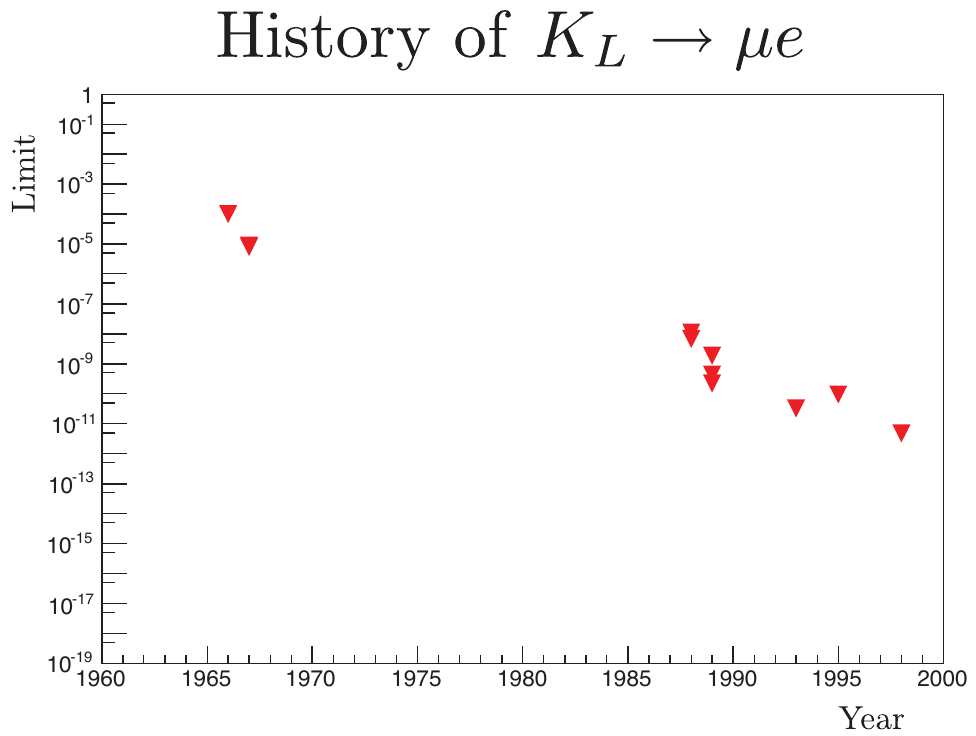
\includegraphics[width =0.4\textwidth]{figures/png/Screenshot_20240307_114258.png}
\caption{.}
\label{fig:Kchannel}
\end{figure}


